\documentclass[aspectratio=169,11pt]{beamer}

\usepackage[T1]{fontenc}
\usepackage{lmodern}
\usepackage{amsmath,amssymb}
\usepackage{booktabs}
\usepackage{graphicx}
\usepackage{xcolor}

\graphicspath{{../Final_Report_Research/pic/generated/}}
\usetheme{Madrid}
\definecolor{researchblue}{RGB}{20,75,115}
\definecolor{researchteal}{RGB}{15,120,125}
\definecolor{researchorange}{RGB}{220,120,40}
\definecolor{softblue}{RGB}{232,242,249}
\definecolor{softred}{RGB}{252,236,236}
\setbeamercolor{structure}{fg=researchblue}
\setbeamercolor{palette primary}{bg=researchblue,fg=white}
\setbeamercolor{palette secondary}{bg=researchteal,fg=white}
\setbeamercolor{palette tertiary}{bg=researchblue!85!black,fg=white}
\setbeamercolor{frametitle}{bg=researchblue,fg=white}
\setbeamercolor{title}{fg=white}
\setbeamercolor{titlelike}{bg=researchblue,fg=white}
\setbeamercolor{block title}{bg=researchblue,fg=white}
\setbeamercolor{block body}{bg=softblue}
\setbeamercolor{block title alerted}{bg=researchorange,fg=white}
\setbeamercolor{block body alerted}{bg=softred}
\setbeamertemplate{navigation symbols}{}
\setbeamertemplate{itemize items}[circle]
\setbeamerfont{frametitle}{size=\large}
\setbeamertemplate{bibliography item}[text]
\newcommand{\source}[1]{\vfill{\tiny\color{gray!80}Source: \cite{#1}}}
\newcommand{\figcaption}[1]{\vspace{0.08cm}{\scriptsize #1}}

\title[MLII ECG]{MLII ECG Anomaly Detection\\and Arrhythmia Classification}
\subtitle{Corrected retrospective temporal evaluation}
\author[A.K.S.S. Wimalasena]{A.K.S.S. Wimalasena}
\institute[University of Ruhuna]{Department of Mathematics\\University of Ruhuna}
\date{Final Research Presentation -- September 2026}

\begin{document}

\begin{frame}[plain]
\titlepage
\vspace{-0.4cm}
\begin{center}\small Supervisor: Ms. Sachini Karunarathne\end{center}
\end{frame}

\begin{frame}{Research question and scope}
Can a single-lead system detect abnormal beats and assign a supported subtype
in later ECG from patients whose earlier ECG was available for training?
\medskip
\begin{itemize}
\item Binary decision: N or abnormal.
\item Conditional subtype: PVC, PAC, LBBB, RBBB or AFib.
\item Targets: whole-system accuracy above 90\%, lower 95\% bound above
90\%, interval width at most three percentage points.
\end{itemize}
\begin{alertblock}{Interpretation}
The temporal test was observed during earlier development.
This is a retrospective known-patient evaluation.
\end{alertblock}
\end{frame}

\begin{frame}{Why morphology and rhythm both matter}
\centering
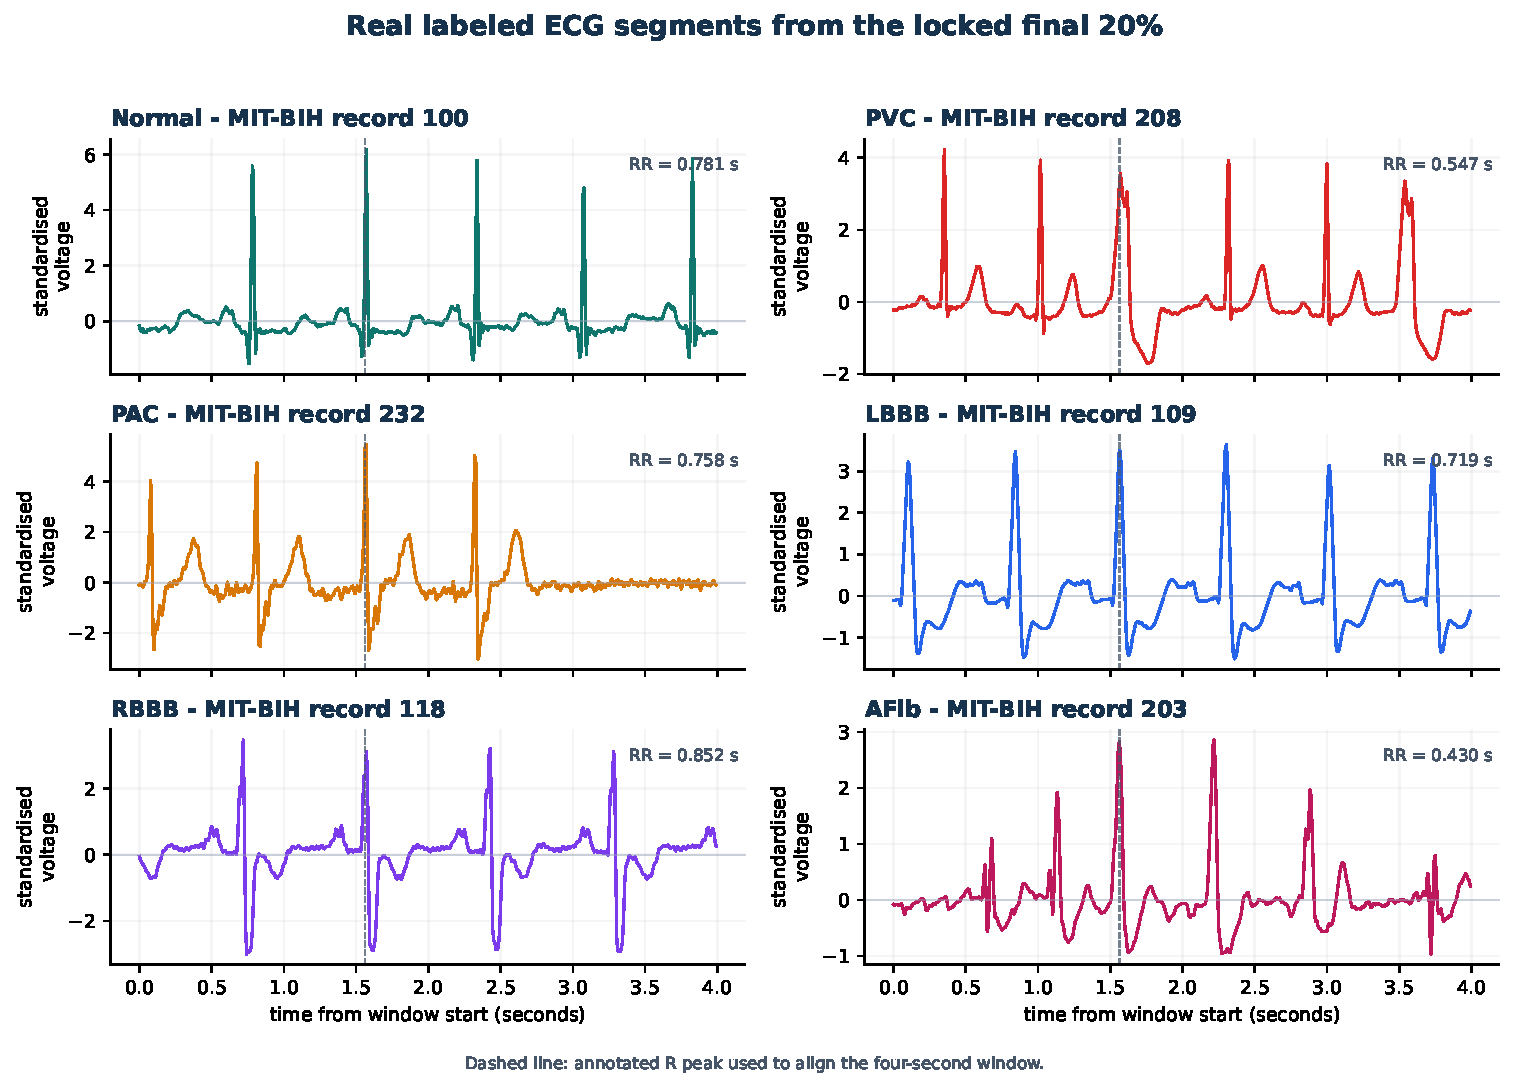
\includegraphics[width=.91\textwidth,height=.68\textheight,keepaspectratio]{real_arrhythmia_examples.pdf}
\figcaption{Illustrative MITDB MLII examples. PVC and bundle-branch patterns
alter shape; premature beats and AF rhythms also require timing context.}
\source{mitdb,dechazal2004heartbeat}
\end{frame}

\begin{frame}{The output codes are annotation groups}
\small
\begin{tabular}{lll}
\toprule
Code & Reference annotation & Interpretation\\
\midrule
N & N, e, j outside AFIB/AFL & Normal-like and escape group\\
PVC & V, E & Ventricular premature/escape\\
PAC & A, a, J, S & Supraventricular premature group\\
LBBB & L & Left bundle-branch beat\\
RBBB & R & Right bundle-branch beat\\
AFib & N-like beat in AFIB/AFL & Fibrillation/flutter context\\
\bottomrule
\end{tabular}
\medskip
Other supported beat symbols keep their morphology label during AFIB/AFL.
Unsupported abnormalities enter binary testing only.
\medskip

These codes are not pure clinical diagnoses or the standard AAMI five classes.
AFib recall is not AF-only or episode-level sensitivity.
\source{mitdb}
\end{frame}

\begin{frame}{Data sources and independent subjects}
\small
\begin{tabular}{lp{.68\textwidth}}
\toprule
Source & Role\\
\midrule
NSRDB & 18 subjects; first stored ECG channel, ECG1.
15 subjects fit the autoencoder; 3 validate it.\\
MITDB & 46 MLII records; 45 subject clusters.
Earlier beats develop the hierarchy; later beats form the temporal test.\\
INCART & Complete cached I01 and I02 recordings, lead II.
Both belong to source patient 1. Post-fit external check only.\\
\bottomrule
\end{tabular}
\medskip
NSRDB has no significant arrhythmias at cohort level; individual windows
were not screened using beat annotations.
\source{nsrdb,mitdb,incartdb}
\end{frame}

\begin{frame}{One channel at each stage}
\begin{itemize}
\item NSRDB ECG1 supplies normal-reference reconstruction; its anatomical
lead is unspecified.
\item MITDB MLII is selected by header name. Record 114 stores it second.
\item Records 102 and 104 lack MLII and are excluded.
\item INCART standard lead II introduces a lead and acquisition shift.
\item The software checks a sensor's declared lead, but cannot verify
physical electrode placement.
\end{itemize}
\source{nsrdb,mitdb,incartdb}
\end{frame}

\begin{frame}{Corrected signal preparation}
\begin{enumerate}
\item Resample the one-channel signal to 128 Hz.
\item Extract 512 samples around an R peak at index 200.
\item Filter within that four-second window: Butterworth 0.5--50 Hz,
forward and backward.
\item Standardise that window to zero mean and unit variance.
\item Require finite, non-flat input and observed previous/next R peaks.
\end{enumerate}
\medskip
The same local preparation now supplies supervised fitting, offline scoring
and streaming classification. This removes the original recording-wide
normalisation and its test-region scale information.
\end{frame}

\begin{frame}{Beat context creates a deliberate delay}
\centering
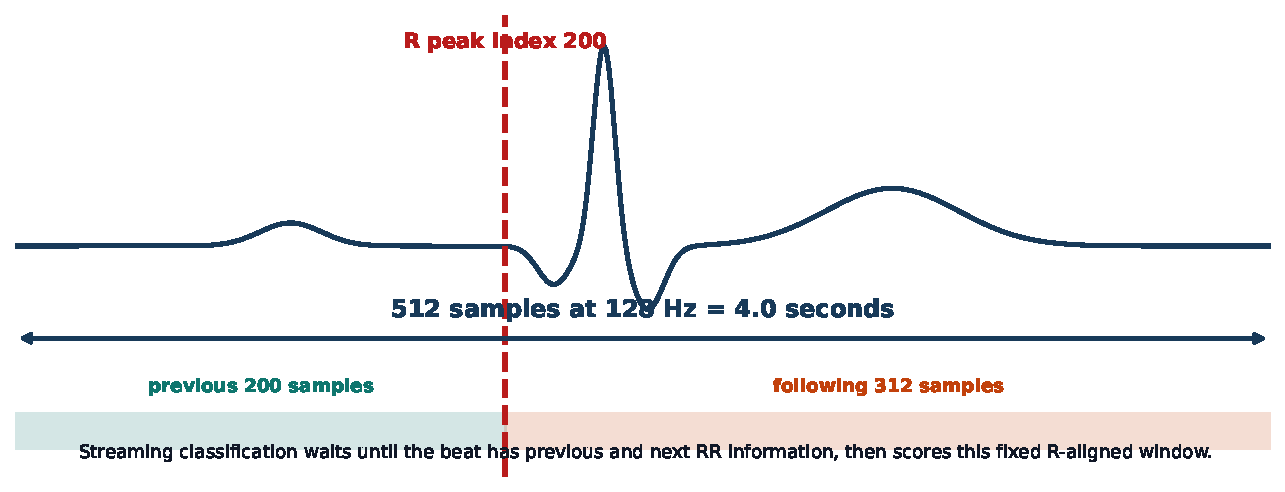
\includegraphics[width=.96\textwidth,height=.60\textheight,keepaspectratio]{architecture_streaming_window.pdf}
\figcaption{A beat needs approximately 2.44 seconds of post-R signal and its
next observed R peak. Chunk buffering and computation add delay.}
\medskip
\small Offline experiments use annotations. Live detection errors and
hardware latency require separate measurement.
\end{frame}

\begin{frame}{Frozen normal-reference autoencoder}
\begin{itemize}
\item Dilated U-Net with residual convolutions and scaled skip connections.
\item 2,680,641 trainable parameters; input and output shape $1\times512$.
\item 288,673 fitting windows and 57,177 validation windows.
\item Two epochs; Adam learning rate 0.001; batch size 256.
\item Denoising noise standard deviation 0.03; best validation MSE 0.061193.
\end{itemize}
\medskip
The checkpoint remains frozen. Two epochs do not establish optimal
convergence, and no ablation establishes the residual branch's independent benefit.
\source{hinton2006autoencoder,vincent2008denoising}
\end{frame}

\begin{frame}{The two ensembles share 242 features}
\begin{tabular}{lr}
\toprule
Feature group & Count\\
\midrule
Whole-window mean bins & 64\\
Central morphology bins & 80\\
Central derivative bins & 60\\
Relative frequency-band powers & 8\\
Signal summary statistics & 11\\
RR timing: 7 base plus 8 historical values & 15\\
Autoencoder reconstruction residuals & 4\\
\midrule
Total & 242\\
\bottomrule
\end{tabular}
\medskip
\small The four residuals are whole-window MAE/MSE, central MAE and
mean absolute residual change.
\end{frame}

\begin{frame}{Hierarchical decision rule}
Let $p_i$ be the ensemble abnormality score and $q_{ic}$ the conditional
subtype score for class $c\in\{1,\ldots,5\}$.
\[
\widehat y_i=
\begin{cases}
0\;(\mathrm{N}) & p_i\leq 0.5708333333,\\
\arg\max_{c\in\{1,\ldots,5\}}q_{ic} & p_i>0.5708333333.
\end{cases}
\]
\begin{itemize}
\item Detector: 240 Extra Trees, square-root feature sampling.
\item Subtype model: 260 Extra Trees, feature sampling 0.33.
\item Both use class/subject weights and entropy splits.
\end{itemize}
\small Every gated beat receives a supported subtype. There is no validated
unknown-class rejection or calibrated disease probability.
\source{geurts2006extratrees}
\end{frame}

\begin{frame}{Chronological split and leakage controls}
\begin{tabular}{lr}
\toprule
Region & Corrected accepted beats\\
\midrule
Candidate training: first 64\%, less gap & 66,285\\
Selection validation: 64--80\%, less gap & 16,029\\
Final refit: first 80\%, less gap & 83,050\\
Temporal test: final 20\% & 20,969\\
\bottomrule
\end{tabular}
\medskip
\begin{itemize}
\item Percentages count accepted beats, not exact elapsed recording time.
\item Remove 16 beats before validation and test boundaries.
\item Check sample separation, including a resampling margin.
\item Test exposure in earlier development remains a source of optimism.
\end{itemize}
\end{frame}

\begin{frame}{Candidate selection uses the development region}
\centering
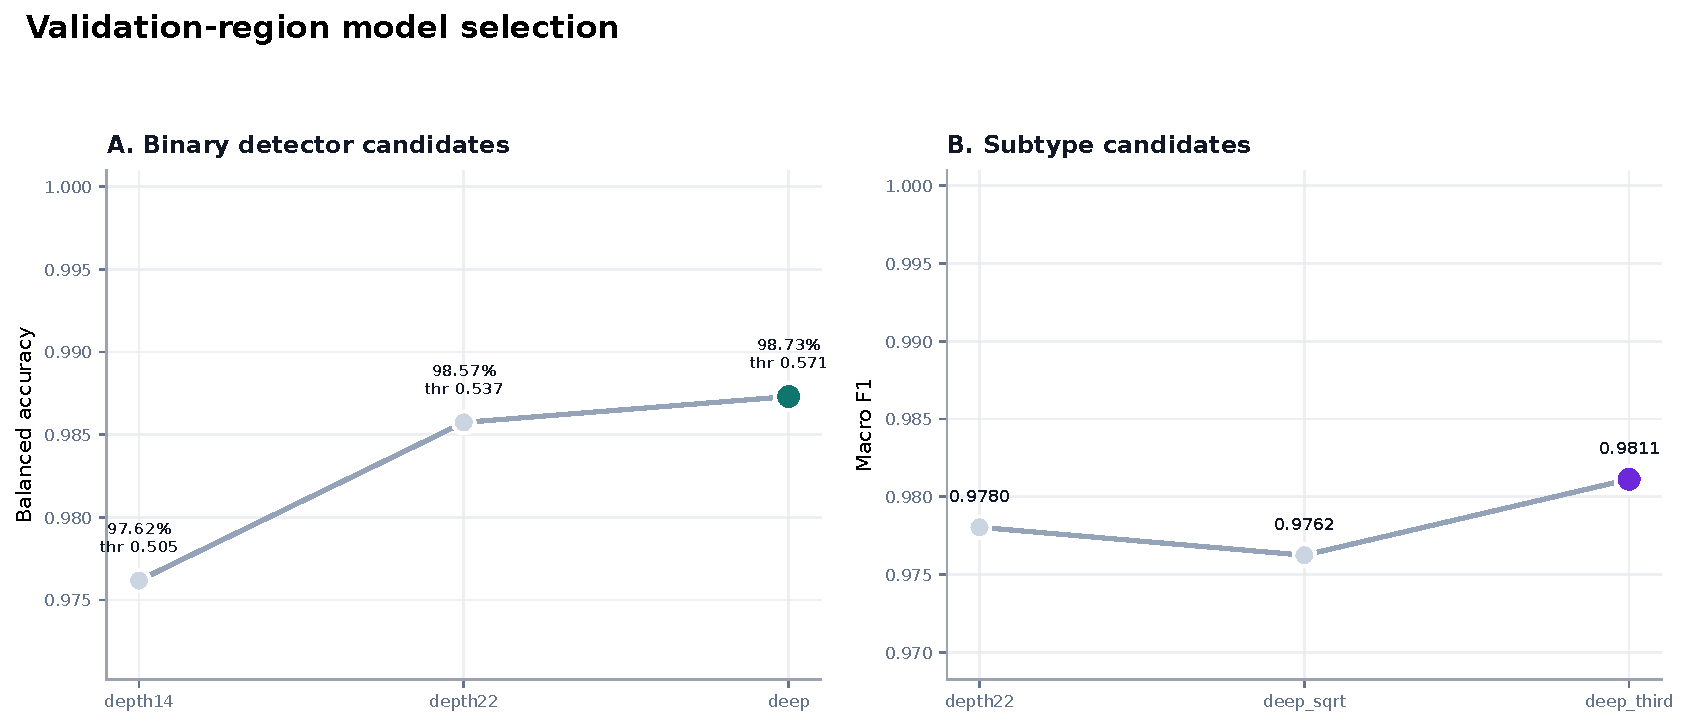
\includegraphics[width=.97\textwidth,height=.67\textheight,keepaspectratio]{method_model_selection.pdf}
\figcaption{Binary candidates rank by balanced accuracy then F1.
Subtype candidates rank by macro F1 then accuracy.
The test does not choose the threshold in this rerun.}
\end{frame}

\begin{frame}{Three evaluations have different denominators}
\begin{tabular}{lrp{.42\textwidth}}
\toprule
Evaluation & Beats & Meaning\\
\midrule
Binary & 20,969 & N versus any accepted abnormality\\
Conditional subtype & 7,958 & True supported abnormalities, ignoring gate\\
Whole system & 20,043 & N plus five supported groups, after gate\\
\bottomrule
\end{tabular}
\medskip
There are 926 unsupported abnormal test beats. They contribute to binary
metrics but not to the six-class confusion matrix.
\medskip

Whole-system accuracy includes correct N outputs and can remain high when a
less common subtype has poor recall.
\end{frame}

\begin{frame}{Corrected temporal whole-system accuracy is 98.07\%}
\centering
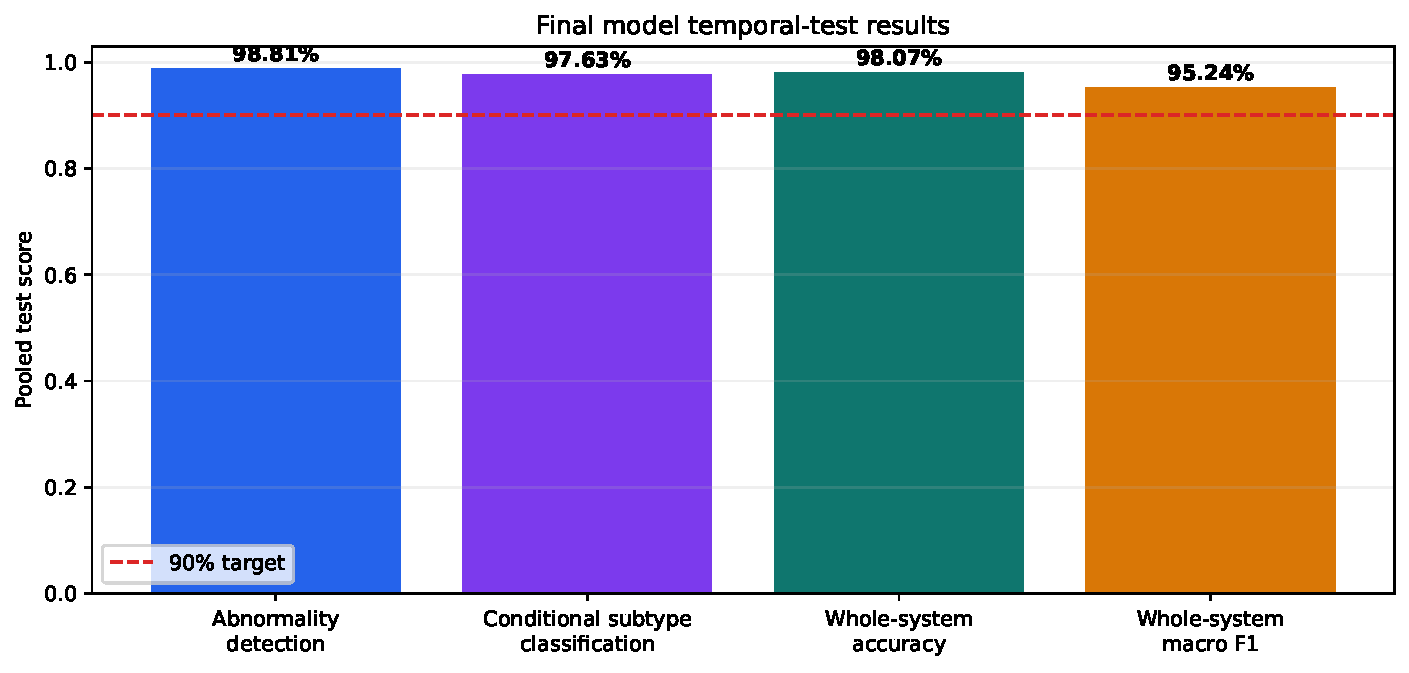
\includegraphics[width=.94\textwidth,height=.68\textheight,keepaspectratio]{final_metrics.pdf}
\figcaption{Binary accuracy 98.81\%; conditional subtype accuracy 97.63\%;
whole-system macro F1 0.9524. Retrospective known-patient results.}
\end{frame}

\begin{frame}{Equal-subject accuracy and uncertainty}
\centering
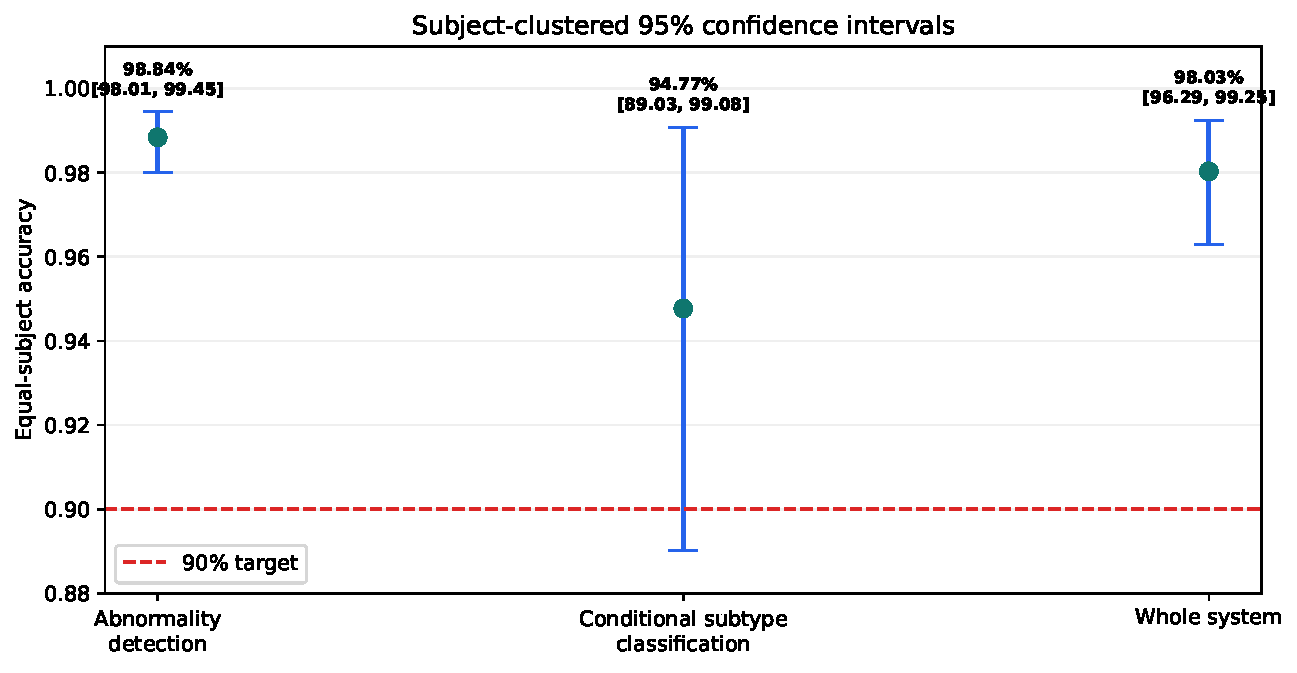
\includegraphics[width=.94\textwidth,height=.68\textheight,keepaspectratio]{final_clustered_ci.pdf}
\figcaption{Whole-system subject mean 98.03\%; 95\% interval 96.29--99.25\%;
width 2.95 percentage points. The interval describes the subject mean,
not pooled accuracy.}
\end{frame}

\begin{frame}{How the confidence interval was calculated}
\begin{enumerate}
\item Combine MITDB records 201 and 202 as one subject.
\item Compute accuracy in each of the 45 subject clusters.
\item Resample 45 clusters with replacement, with equal subject weight.
\item Repeat 10,000 times; take the 2.5th and 97.5th percentiles.
\end{enumerate}
\medskip
The fitted model stays fixed. The interval does not include retraining
variability, development-selection bias or a new population shift.
\medskip

43 of 45 clusters exceed 90\%. The sign test concerns the fraction of
subjects above the target, not pooled beat accuracy.
\source{rutter2000clustered}
\end{frame}

\begin{frame}{PAC recall remains below the target}
\small
\begin{tabular}{lrrrr}
\toprule
Group & True & Correct & Precision & Recall\\
\midrule
PVC & 1,527 & 1,499 & 92.36\% & 98.17\%\\
PAC & 589 & 416 & 98.58\% & 70.63\%\\
LBBB & 1,481 & 1,476 & 96.72\% & 99.66\%\\
RBBB & 1,383 & 1,365 & 99.78\% & 98.70\%\\
AFib group & 2,978 & 2,879 & 98.26\% & 96.68\%\\
\bottomrule
\end{tabular}
\medskip
549 PAC beats pass the gate; 441 are correctly named without gating;
416 are correct end to end.
\medskip

These are annotation-group recalls, not patient diagnoses.
\end{frame}

\begin{frame}{Whole-system errors}
\centering
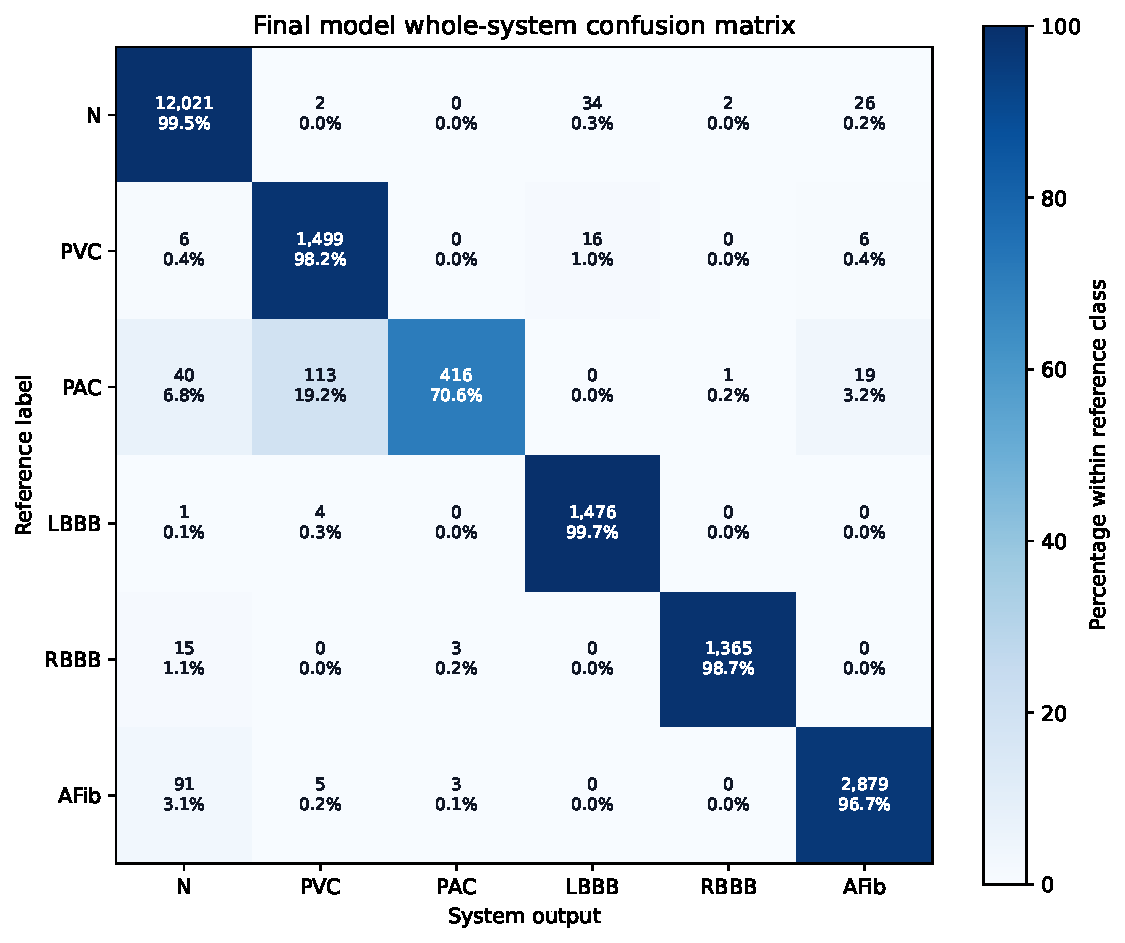
\includegraphics[width=.78\textwidth,height=.74\textheight,keepaspectratio]{final_confusion_matrix.pdf}
\figcaption{113 PAC beats become PVC. The gate sends 91 AFib-group beats and
40 PAC beats to N.}
\end{frame}

\begin{frame}{External check covers one INCART source patient}
\small
\begin{tabular}{lr}
\toprule
Fixed post-fit check & Result\\
\midrule
I01 and I02; both patient 1 & 5,416 beats\\
Reference N / PVC & 4,845 / 571\\
Binary accuracy / balanced accuracy & 94.11\% / 96.55\%\\
Sensitivity / specificity & 99.65\% / 93.46\%\\
Binary precision & 64.22\%\\
False alarms / missed abnormalities & 317 / 2\\
Whole-system accuracy & 92.85\%\\
End-to-end PVC recall & 87.74\%\\
\bottomrule
\end{tabular}
\medskip
The threshold stays fixed. The subset has no reference support for PAC,
LBBB, RBBB or AFib and cannot establish population generalisation.
\source{incartdb}
\end{frame}

\begin{frame}{What the prototype establishes}
\begin{itemize}
\item A working single-lead hierarchy with reproducible preparation and scoring.
\item Aggregate accuracy, lower confidence bound and interval-width targets
met in the retrospective temporal run.
\item Persistent PAC weakness and external false alarms.
\item Consistent offline/streaming feature construction when peak locations agree.
\end{itemize}
\begin{alertblock}{What remains unvalidated}
An untouched patient-disjoint test, all-class external recall, real AD8232
performance, clinical signal quality and prospective use.
\end{alertblock}
\end{frame}

\begin{frame}{Research limitations and next study}
\begin{itemize}
\item Earlier test exposure can bias design choices; the rerun cannot undo it.
\item The NSRDB channel differs from MLII, and normality is a cohort assumption.
\item The autoencoder's added value needs a controlled ablation.
\item Labels combine beat morphology and rhythm context.
\item A new study must reserve independent patients before any model selection.
\item Sensor validation must measure peak detection, false alarms and total latency.
\end{itemize}
\end{frame}

\begin{frame}{Conclusion}
The corrected hierarchy reaches 98.07\% whole-system accuracy on the
retrospective MITDB temporal test, with an equal-subject 95\% interval of
96.29--99.25\%.
\medskip

PAC recall remains 70.63\%. The one-patient INCART check shows 92.85\%
whole-system accuracy and substantial false alarms.
\medskip

The research contribution is a reproducible prototype with explicit
evaluation limits. Clinical diagnostic performance has not been established.
\end{frame}

\appendix
\begin{frame}{Technical detail: actual autoencoder tensor sizes}
\small
\begin{tabular}{ll}
\toprule
Stage & Channels $\times$ samples\\
\midrule
Input & $1\times512$\\
Encoder blocks & $32\times256,\ 64\times128,\ 128\times64,\ 256\times32$\\
Dilated bottleneck & $256\times32$; dilations 1, 2, 4, 8\\
Decoder after skip resizing & $128\times32,\ 64\times64,\ 32\times128,\ 32\times256$\\
Linear output then interpolation & $1\times256$ then $1\times512$\\
\bottomrule
\end{tabular}
\medskip
The first up block resizes to its length-32 skip. A final interpolation
restores the input length. The diagram and report describe the saved
implementation, not an idealised doubling at every decoder stage.
\end{frame}

\begin{frame}{Technical detail: residual and RR features}
\small
With $e_t=x_t-\hat x_t$, the four residuals are
\[
\frac1{512}\sum|e_t|,\quad \frac1{512}\sum e_t^2,\quad
\frac1{240}\sum_{t=104}^{343}|e_t|,\quad
\frac1{511}\sum_{t=1}^{511}|e_t-e_{t-1}|.
\]
The seven base RR values describe previous/next interval, local mean,
interval ratios, local variation and heart rate.
\medskip

The eight historical values use up to 20 completed intervals: median,
IQR, MAD, RMSSD, pNN50, relative range, trend and latest change.
Only the next-RR base features require the next beat.
\end{frame}

\begin{frame}{Technical detail: class and subject weights}
For class $c$ and subject cluster $s$,
\[
w_{cs}\propto \frac1{n_c}
\left(\frac{n_c}{S_c n_{cs}}\right)^\alpha .
\]
\begin{itemize}
\item $n_c$: class support; $S_c$: subjects containing the class.
\item $n_{cs}$: beats of class $c$ in subject cluster $s$.
\item Normalise weights to mean one and clip to $[0.05,20]$.
\item Selected $\alpha$: 0.35 for binary, 0.25 for subtype.
\end{itemize}
Records 201 and 202 form one cluster during weighting and uncertainty analysis.
\end{frame}

\begin{frame}[allowframebreaks]{References}
\footnotesize
\bibliographystyle{ieeetr}
\bibliography{refe}
\end{frame}
\end{document}
